\chapter{Two-source refractive index measurement}
\label{chap:refractive_index}

\section{Introduction}
\label{intro_ts}
In chapter \ref{chap:two_source}, the $0-\pi$ square-wave phase grating (SWPG) was introduced as a means of generating two intense duplicates of an input femtosecond mid-IR pulse.  An additional element of the SWPG is that it enables precise control over the relative phase between these two sources.  When used to generate high harmonics, this scheme enables the generation of two XUV sources whose relative phase is well controlled by the SWPG, and any small phase shift between the two harmonic beams is imprinited upon their interference pattern as a phase shift in the far-field.  The idea is to now leverage this sensitivity to measure an induced phase shift between the two XUV sources.  In the experiment described in this chapter, the phase shift will be induced by introducing a thin condensed matter sample into only one of the two XUV sources.  Doing so enables us to extract both the real and imaginary part of the refractive index over a broad range of photon energies in the XUV.
\section{Complex refractive index}
The complex refractive index in the XUV range depends strongly on photon energy. In this energy region there are many resonances that correspond to transitions of core-level electrons to unoccupied states near the Fermi level (for the case of a condensed matter system)\cite{stohrNEXAFSSpectroscopy1992}.  Complicated fine structure can emerge near these resonances that correspond to the local electronic and geometric environment\cite{stohrNEXAFSSpectroscopy1992}.  Thus, the ability to measure both the real and imaginary parts of the complex refractive index can be important for many experiements using XUV light generated by HHG\cite{kaplanFemtosecondTrackingCarrier2018,  cirriAchievingSurfaceSensitivity2017}.

\begin{figure}
	\centering
	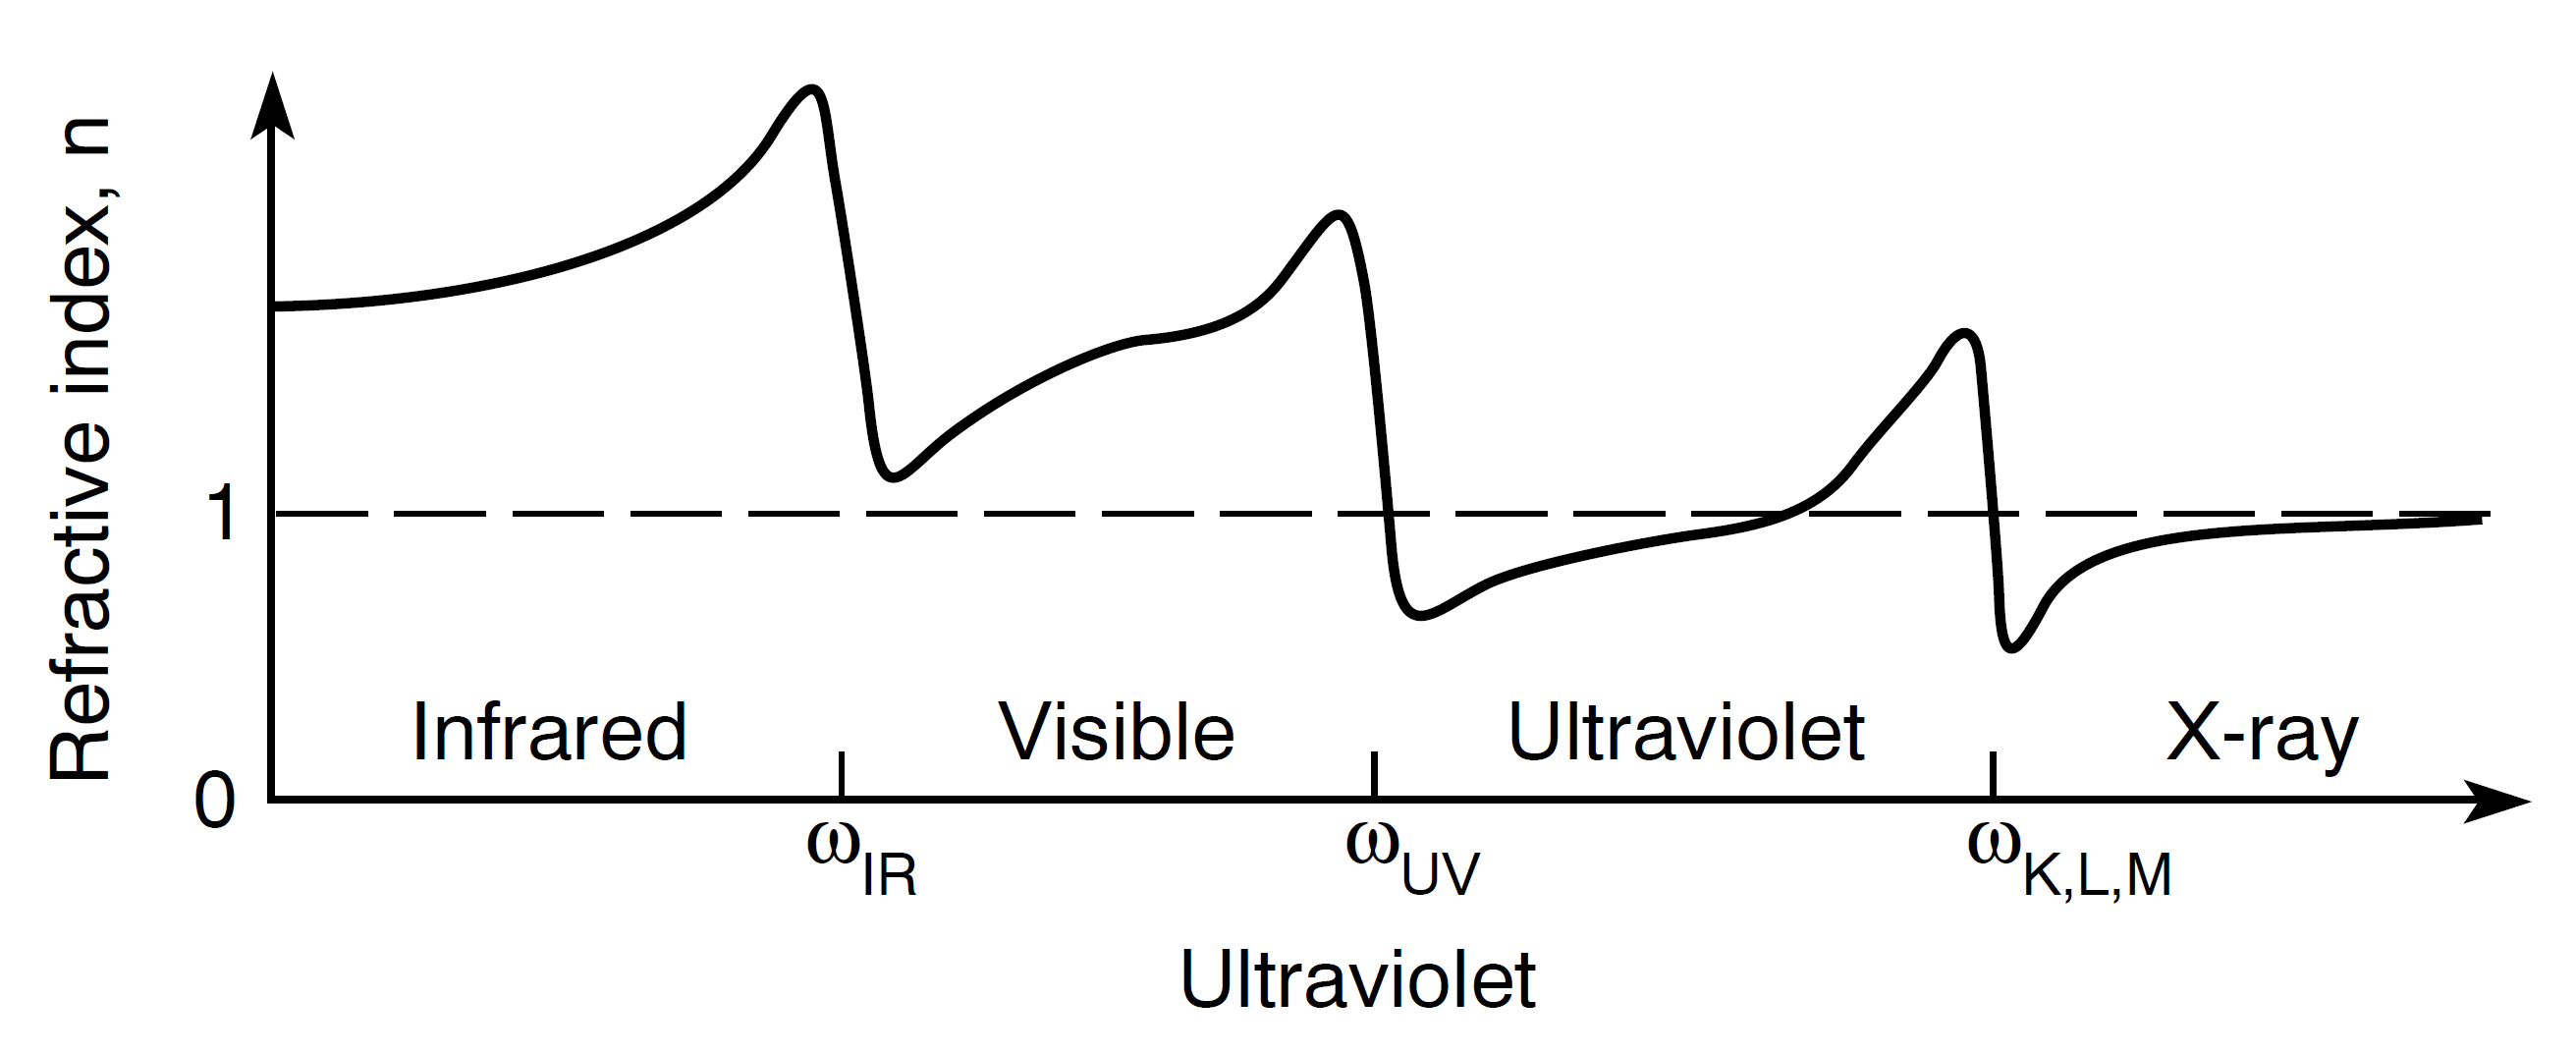
\includegraphics[width=0.7\textwidth]{figures/refractive_index/attwood_real_n_schematic.png}
	\caption{Schematic of the real part of the refractive index versus photon energy. Example resonances are shown in the IR, the visible/UV, and in the XUV/soft x-ray regimes. In general, the refractive index approaches 1 at higher photon energies.  Adapted from \cite{attwoodSoftXraysExtreme2000}.}
	\label{fig:refractive_index_schematic}
\end{figure}

In general, the complex refractive index can be written as\cite{attwoodSoftXraysExtreme2000}
\begin{equation}
\label{eqn:refractive_index}
	n(\omega)=1 - \bigg(\frac{n_a r_e \lambda^2}{2\pi}\bigg)\bigg[f_1(\omega) - i f_2(\omega)\bigg]
\end{equation}
where $n_a$ is the number density, $\omega$ ($\lambda$) is the photon energy (wavelength), and
\begin{equation}
\label{eqn:r_e}
	r_e = \frac{e^2}{4\pi\epsilon_0 mc^2}
\end{equation}
is the classical electron radius. By introducing the parameters $\beta$ and $\delta$, such that
\begin{equation}
\label{eqn:delta_beta_def}
	\begin{aligned}
	\delta &= \frac{n_a r_e \lambda^2}{2\pi}f_1(\omega)
	\beta & = \frac{n_a r_e \lambda^2}{2\pi}f_2(\omega),
	\end{aligned}
\end{equation}
then the refractive index $n$ can be written as
\begin{equation}
\label{eqn:refractive_index_db}
	n(\omega)=1-\delta+i\beta.
\end{equation}
The values of both $\delta$ and $\beta$ have been tabulated for elements from hydrogen up to uranium in the range of 10 eV to 30 keV\cite{henkeLowenergyXrayInteraction1982}.  Values for $\delta$ and $\beta$ are generally smaller than unity when far from resonance.

Now that we've established the form of the refractive index, we will consider the case of propagation through a dispersive medium. The idea\footnote{This discussion closely follows from the textbook by D. Attwood \cite{attwoodSoftXraysExtreme2000}.} is to consider a plane wave of the form
\begin{equation}
	\mathbf{E}(\mathbf{r},t)=\mathbf{E}_0e^{-i(\omega t - \mathbf{k}\cdot\mathbf{r})},
\end{equation}
and assume that the dispersion of the medium takes the form
\begin{equation}
	\frac{\omega}{k}=\frac{c}{n}=\frac{c}{1-\delta+i\beta}.
\end{equation}
With these relationships, one can write the field in the propagation direction defined by $\mathbf{k}\cdot\mathbf{r}=kr$ as
\begin{equation}
	\mathbf{E}(\mathbf{r},t)=\big(e^{-i\omega(t - r/c)}\big) \big(e^{-i(2\pi\delta/\lambda)r}\big) \big(e^{-(2\pi\beta/\lambda)r}\big).
\end{equation}
The first term in parentheses is the vacuum propagation of the wave, the second term is a phase shift proportional to $\beta$ that is induced by the dispersive medium, and the third term is a decay in amplitude that is proportional to $\delta$.  From this relationship, it can be shown that the attenuation of the intensity is given by 
\begin{equation}
\label{eqn:beer-lambert}
	\frac{I}{I_0}=e^{-(4\pi\beta/\lambda)r}=e^{-n_a \sigma_a r}
\end{equation}
where $I_0$ is the initial intensity and $\sigma_a=2r_\lambda f_2(\omega)$ is the photoabsorption cross section.  This relationship shows that by measuring the absorption of a material (a thin film for these photon energies), one can easily extract the imaginary part of the refractive index.

The effect of the real part of the refractive index is to induce a phase shift in propagating field, as can be seen from equation \ref{eqn:beer-lambert}.  After propagating through a material of thickness $L$, the induced phase shift is given by
\begin{equation}
\label{eqn:phase_shift}
	\Delta\phi=\frac{2\pi\delta L}{\lambda}.
\end{equation}
To experimentally access this phase shift, the technique that can be used is interferometry. The idea is to create a Mach-Zehnder interferometer, and in one of the arms introduce a sample of thickness $L$. By measuring how the interference patterns shift when introducing the sample, then one can directly measure the phase shift induced by the sample.  Additionally, by looking how the fringe contrast changes, one can also get access to the attenuation caused by the sample.  This means that both the real and imaginary parts of the refractive index can be probed simultaneously.  This concept is precisely what will be used to extract the real and imaginary parts using the two XUV sources generated by a SWPG.  In that case each source will act as one arm of a Mach-Zehnder interferometer.
\begin{figure}
	\centering
	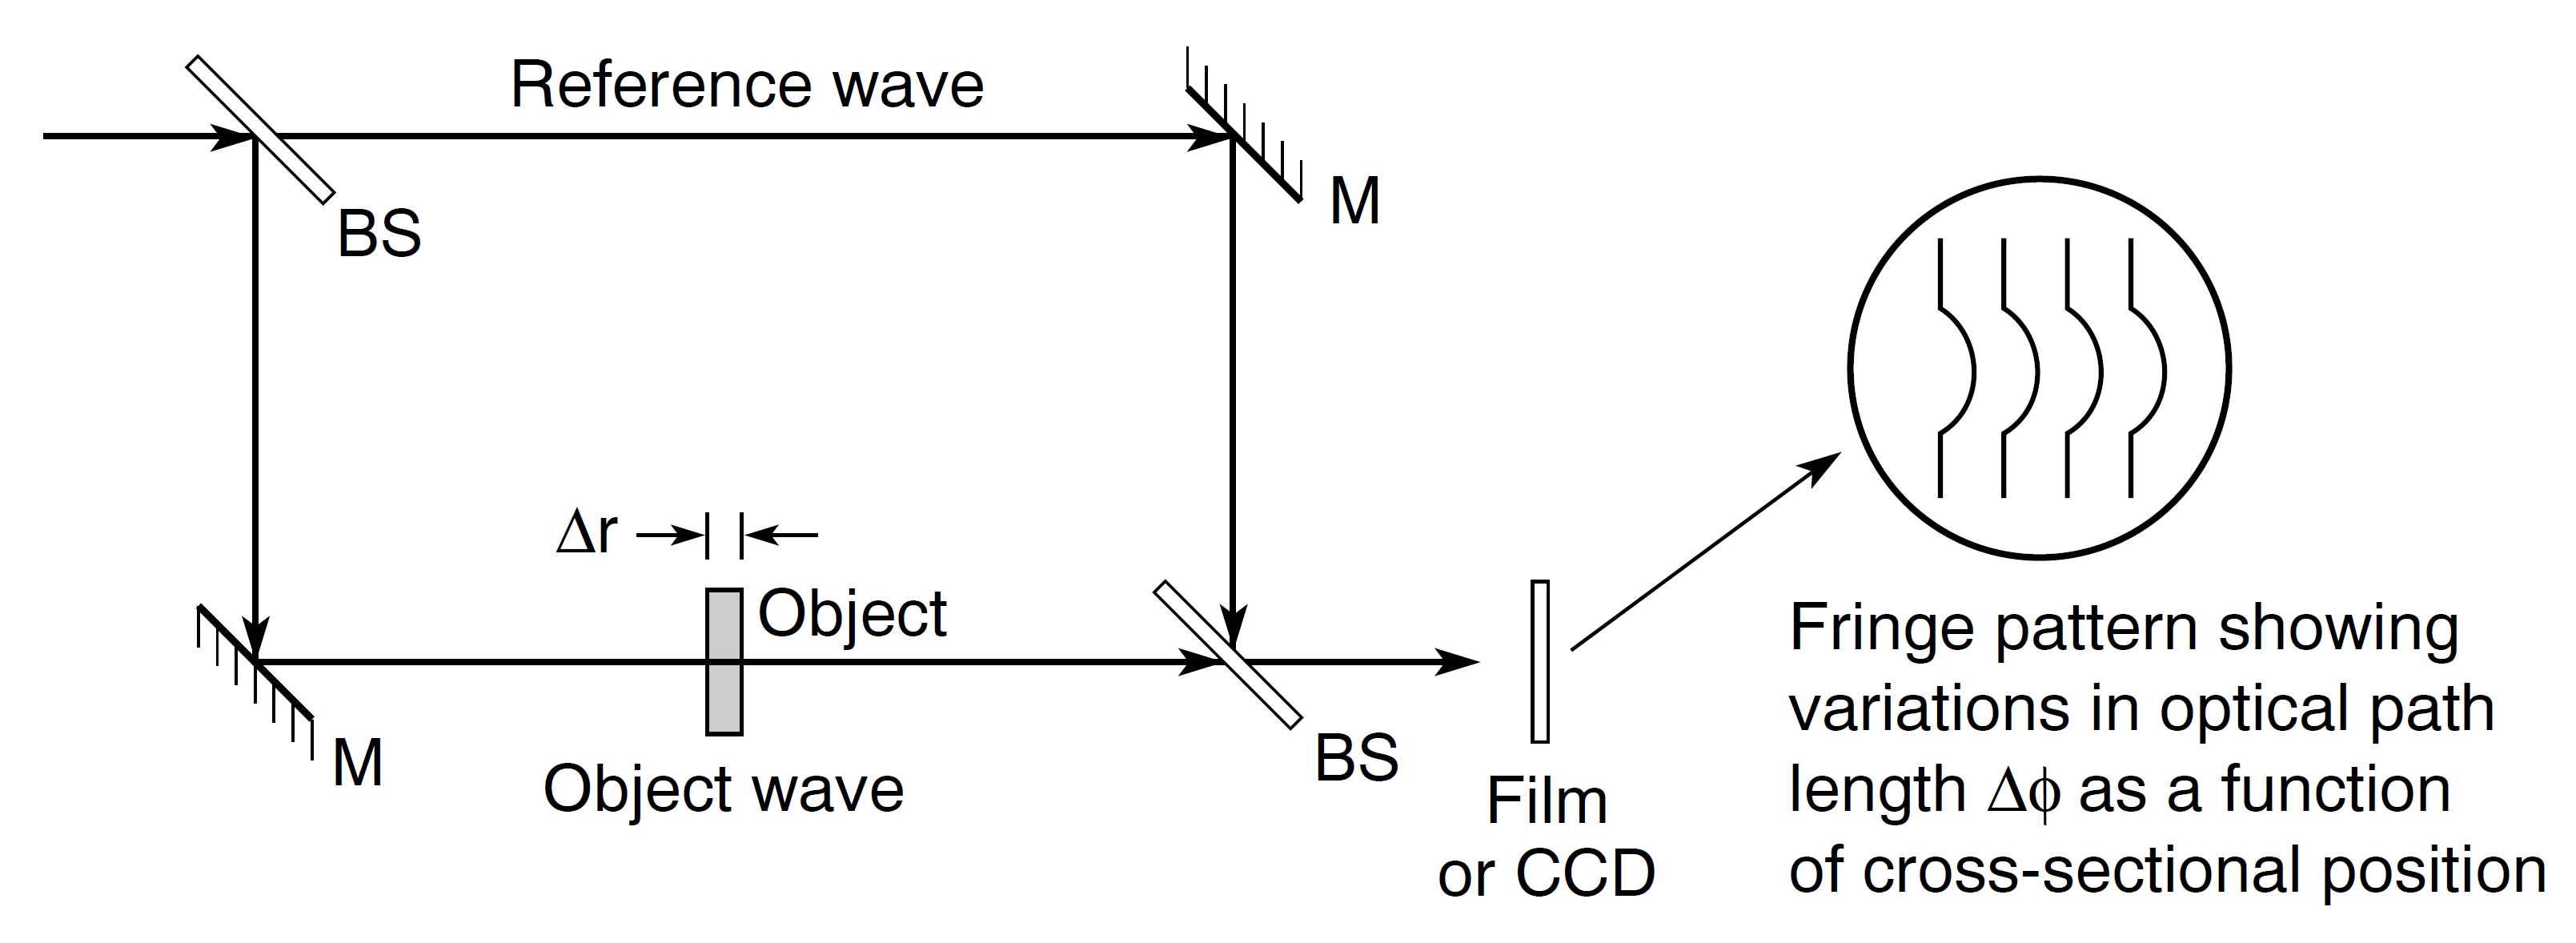
\includegraphics[width=0.7\textwidth]{figures/refractive_index/mach_zehnder_phase_shift.png}
	\caption{Schematic of a Mach-Zehnder interferometer that is used to measure the phase shift induced by a sample placed in one of the arms of the interferometer.  For the experiments described in this chapter, the two XUV sources will act as the two arms of a Mach-Zehnder.  Adapted from \cite{attwoodSoftXraysExtreme2000}.}
	\label{fig:mach-zehnder_interferometer}
\end{figure}

\section{Experimental setup}
\label{sec:experimental_setup_refrac}

